\documentclass[11pt]{article}
\usepackage{setspace}
\usepackage{fullpage}
\usepackage{pslatex}
\usepackage{pgfplots}
\pgfplotsset{
	compat=1.4}
\usepackage{tikz}
\usetikzlibrary{shapes,arrows}
\let\word=\textit
\begin{document}
\begin{figure}[htb]
\centering
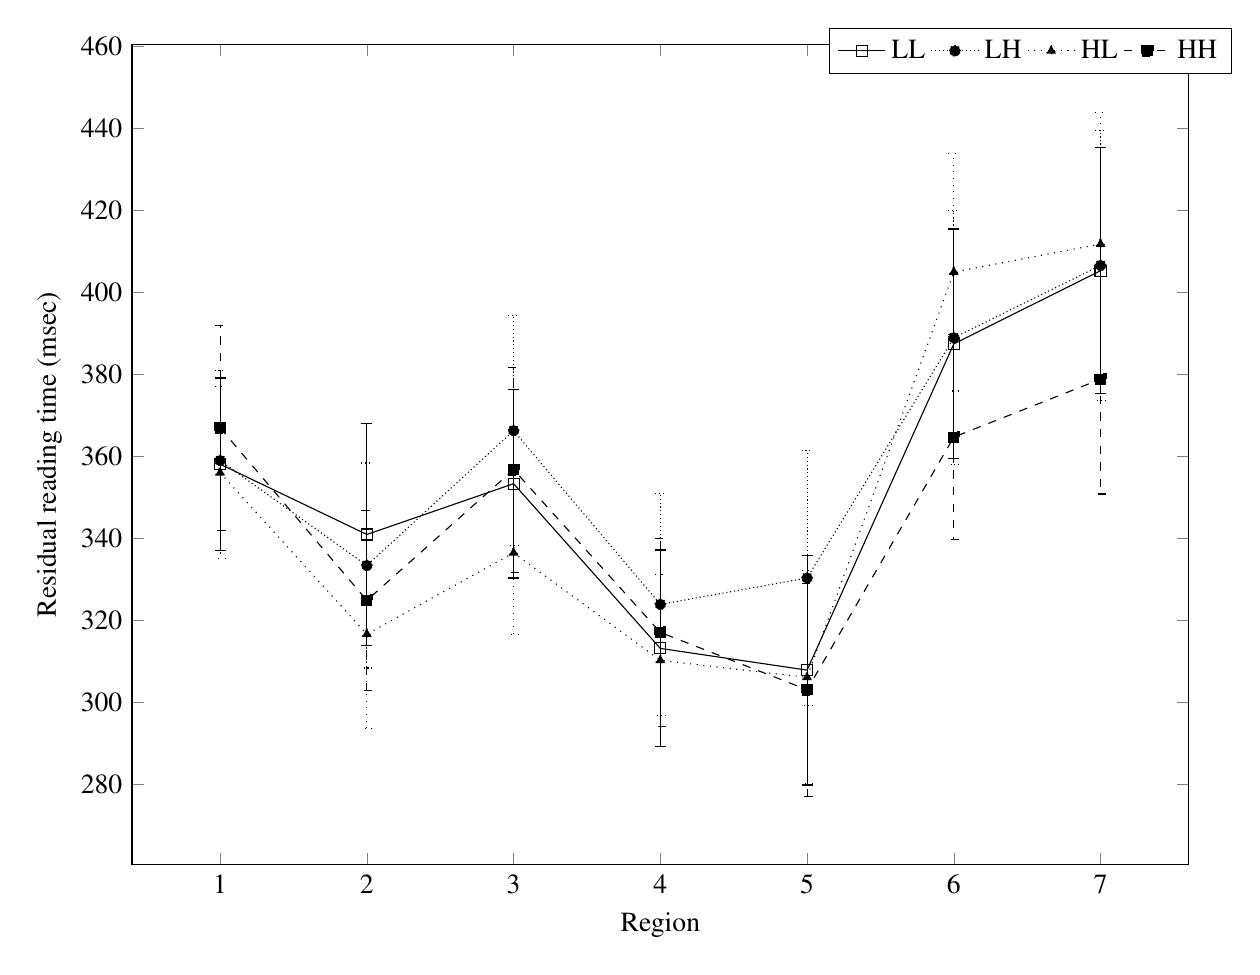
\begin{tikzpicture}
\begin{axis}[
	width=15cm, height=12cm,
	legend style={at={(0.85,1.02)},
	anchor=north,legend columns=-1},
	ylabel={Residual reading time (msec)},
	xlabel={Region},
	symbolic x coords={1, 2, 3, 4, 5, 6, 7},
    	xtick=data,
]
\addplot[
		mark=square,
		error bars/.cd,
		error bar style={color=black},
		y dir=both,
		y explicit
] 
	coordinates {(1, 358.1703 ) +- ( 21 , 21 )(2, 341.02 ) +- ( 27 , 27 )(3, 353.4023 ) +- ( 23 , 23 )(4, 313.2394 ) +- ( 24 , 24 )(5, 307.9428 ) +- ( 28 , 28 )(6, 387.507 ) +- ( 28 , 28 )(7, 405.3467 ) +- ( 30 , 30 )};
\addplot[
		mark=*,
		densely dotted,
		error bars/.cd,
		error bar style={color=black},
		y dir=both,
		y explicit
] 
	coordinates {(1, 359.04 ) +- ( 22 , 22 )(2, 333.4597 ) +- ( 25 , 25 )(3, 366.3432 ) +- ( 28 , 28 )(4, 323.974 ) +- ( 27 , 27 )(5, 330.4099 ) +- ( 31 , 31 )(6, 388.9908 ) +- ( 31 , 31 )(7, 406.6205 ) +- ( 33 , 33 )};
\addplot[
		mark=triangle*,
		dotted,
		error bars/.cd,
		error bar style={color=black},
		y dir=both,
		y explicit
] 
	coordinates {(1, 356.0645 ) +- ( 21 , 21 )(2, 316.7122 ) +- ( 23 , 23 )(3, 336.5534 ) +- ( 20 , 20 )(4, 310.3318 ) +- ( 21 , 21 )(5, 306.1665 ) +- ( 26 , 26 )(6, 405.017 ) +- ( 29 , 29 )(7, 411.8542 ) +- ( 32 , 32 )};
\addplot[
		mark=square*,
		dashed,
		error bars/.cd,
		error bar style={color=black},
		y dir=both,
		y explicit
] 	
    coordinates {(1, 367.0301 ) +- ( 25 , 25 )(2, 324.9553 ) +- ( 22 , 22 )(3, 356.839 ) +- ( 25 , 25 )(4, 317.1446 ) +- ( 23 , 23 )(5, 303.1554 ) +- ( 26 , 26 )(6, 364.7678 ) +- ( 25 , 25 )(7, 378.8816 ) +- ( 28 , 28 )};
\legend{LL,LH,HL,HH}
\end{axis}
\end{tikzpicture}
\caption{Mean residual reading times for all sentence regions}
\end{figure}
\end{document}